\chapter{Experiment} % Main chapter title

\label{Chapter4} % Change X to a consecutive number; for referencing this chapter elsewhere, use \ref{ChapterX}



%----------------------------------------------------------------------------------------
%	SECTION 1
%----------------------------------------------------------------------------------------



To evaluate the effectiveness and practicality of the developed wearable haptic glove, I conducted two structured experiments focusing on both perceptual discrimination and subjective realism of vibrotactile feedback. 
In Experiment 1, I assessed participants' ability to distinguish between three distinct vibration cycle rates delivered through the glove. 
In Experiment 2, I investigated the relationship between the vibration cycle rates and the perceived realism of various virtual textures. 
Together, these experiments provided both quantitative performance data and qualitative user feedback, offering a comprehensive evaluation of the glove’s performance in enhancing virtual texture perception and supporting natural hand interactions in virtual reality applications.

\section{Equipment and Specifications}
The experimental setup included a desktop host machine with an Intel® Core™ i7-13700 processor, an NVIDIA® GeForce RTX™ 3050 graphics card, and 16 GB of system memory. This configuration provided adequate computational power for rendering real-time virtual environments and processing haptic feedback with low latency. The virtual environment was developed using Unity 2022.3.23f1 (LTS), which offered a stable platform for implementing custom interactions and integrating external hardware devices.

The wearable haptic glove, developed in this study, was connected to the host system. The glove’s onboard microcontroller handled real-time sensor data acquisition and vibration control, while Unity managed virtual object interactions and feedback synchronization. This combination of hardware and software provided a responsive and immersive environment for evaluating virtual texture perception and gesture-based control in virtual reality, shown in Fig.~\ref{fig:unity} and Fig.~\ref{fig:experiment}.

\begin{figure}[H]\centering
	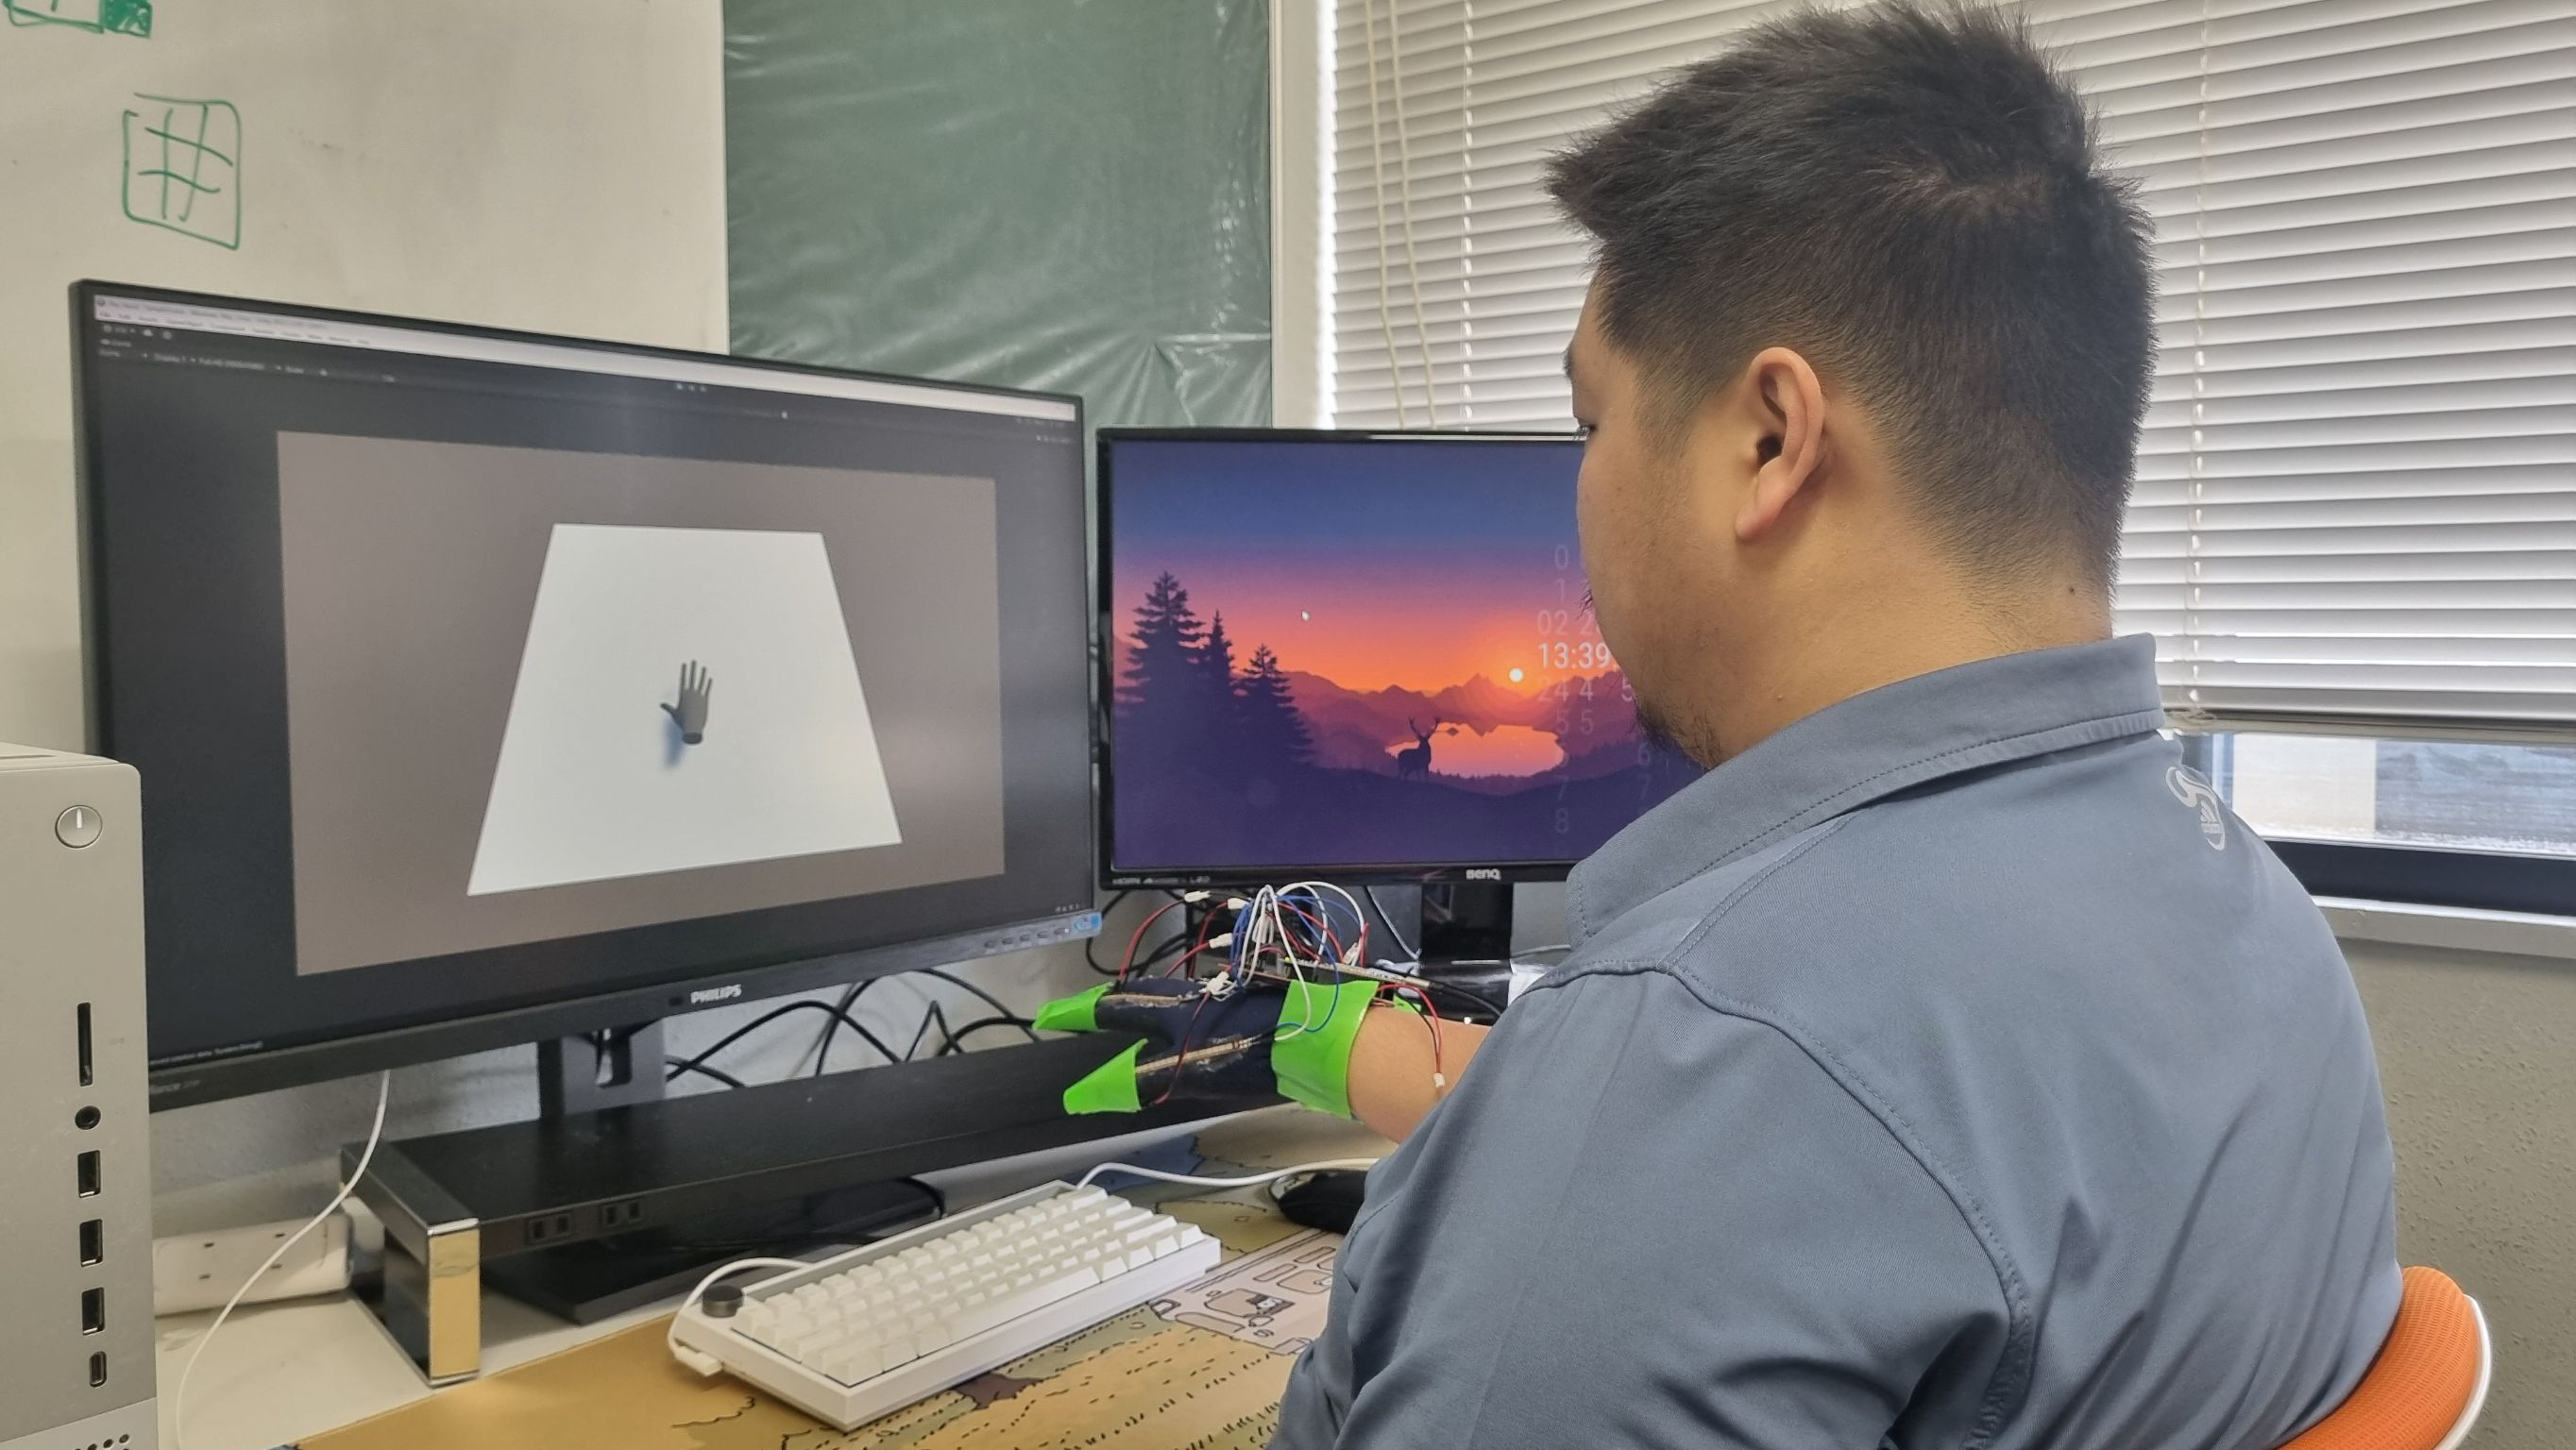
\includegraphics[width=0.9\textwidth]{Pictures/experiment.png}%imagine location
	\caption{Overall experimental setup demonstrating participant interaction using the wearable haptic glove.}\label{fig:experiment}%use name for ref.
	
\end{figure}
%%%%%%%%

\newpage
\section{Haptic Feedback Method}

In this experiment, the haptic feedback method utilizes PWM (Fig.~\ref{fig:pwm_2}) to create vibrotactile sensations that simulate variations in surface texture within virtual environments. The goal of this feedback mechanism is to provide tactile cues that represent different levels of surface granularity, thereby increasing the realism of virtual interactions. This section outlines the signal generation process, cycle rate configuration, vibration pattern design, and how these elements are integrated into the overall virtual reality system.

\begin{figure}[H]\centering
	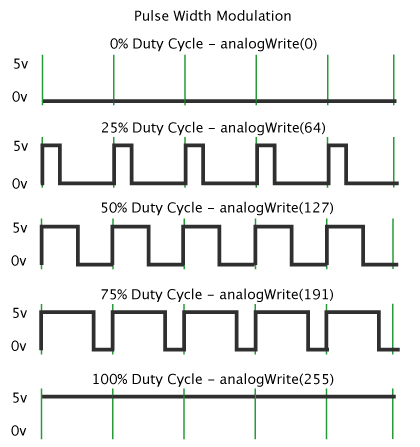
\includegraphics[width=0.7\textwidth]{Pictures/PWM_2.png}%imagine location
	\caption{PWM behavior.~\cite{pwm_doc}}\label{fig:pwm_2}%use name for ref.
	
\end{figure}

\subsubsection{PWM-Based Vibration Control}
PWM is a method of signal modulation in which a digital output rapidly switches between on and off states. The duration for which the signal is in the "on" state during each cycle, known as the duty cycle, determines the effective power delivered to the actuator. In this system, the ESP32 microcontroller generates PWM signals through its dedicated hardware PWM channels. This ensures high-frequency, low-latency signal control, making it suitable for real-time virtual reality applications.

\newpage
\subsubsection{Duty Cycle Settings}
In Fig.~\ref{fig:pwm_3}, the duty cycle was set to fixed values of 0.2, 0.5, and 1.0 to ensure a consistent vibration intensity during each active phase. Preliminary testing revealed that maintaining a constant duty cycle allowed the vibration motor to achieve a noticeable amplitude without causing discomfort. This method helps avoid the variability in perceived intensity that can arise from fluctuating duty cycles, enabling the study to concentrate solely on the effects of vibration rhythm and cycle rate.

\begin{figure}[H]\centering
	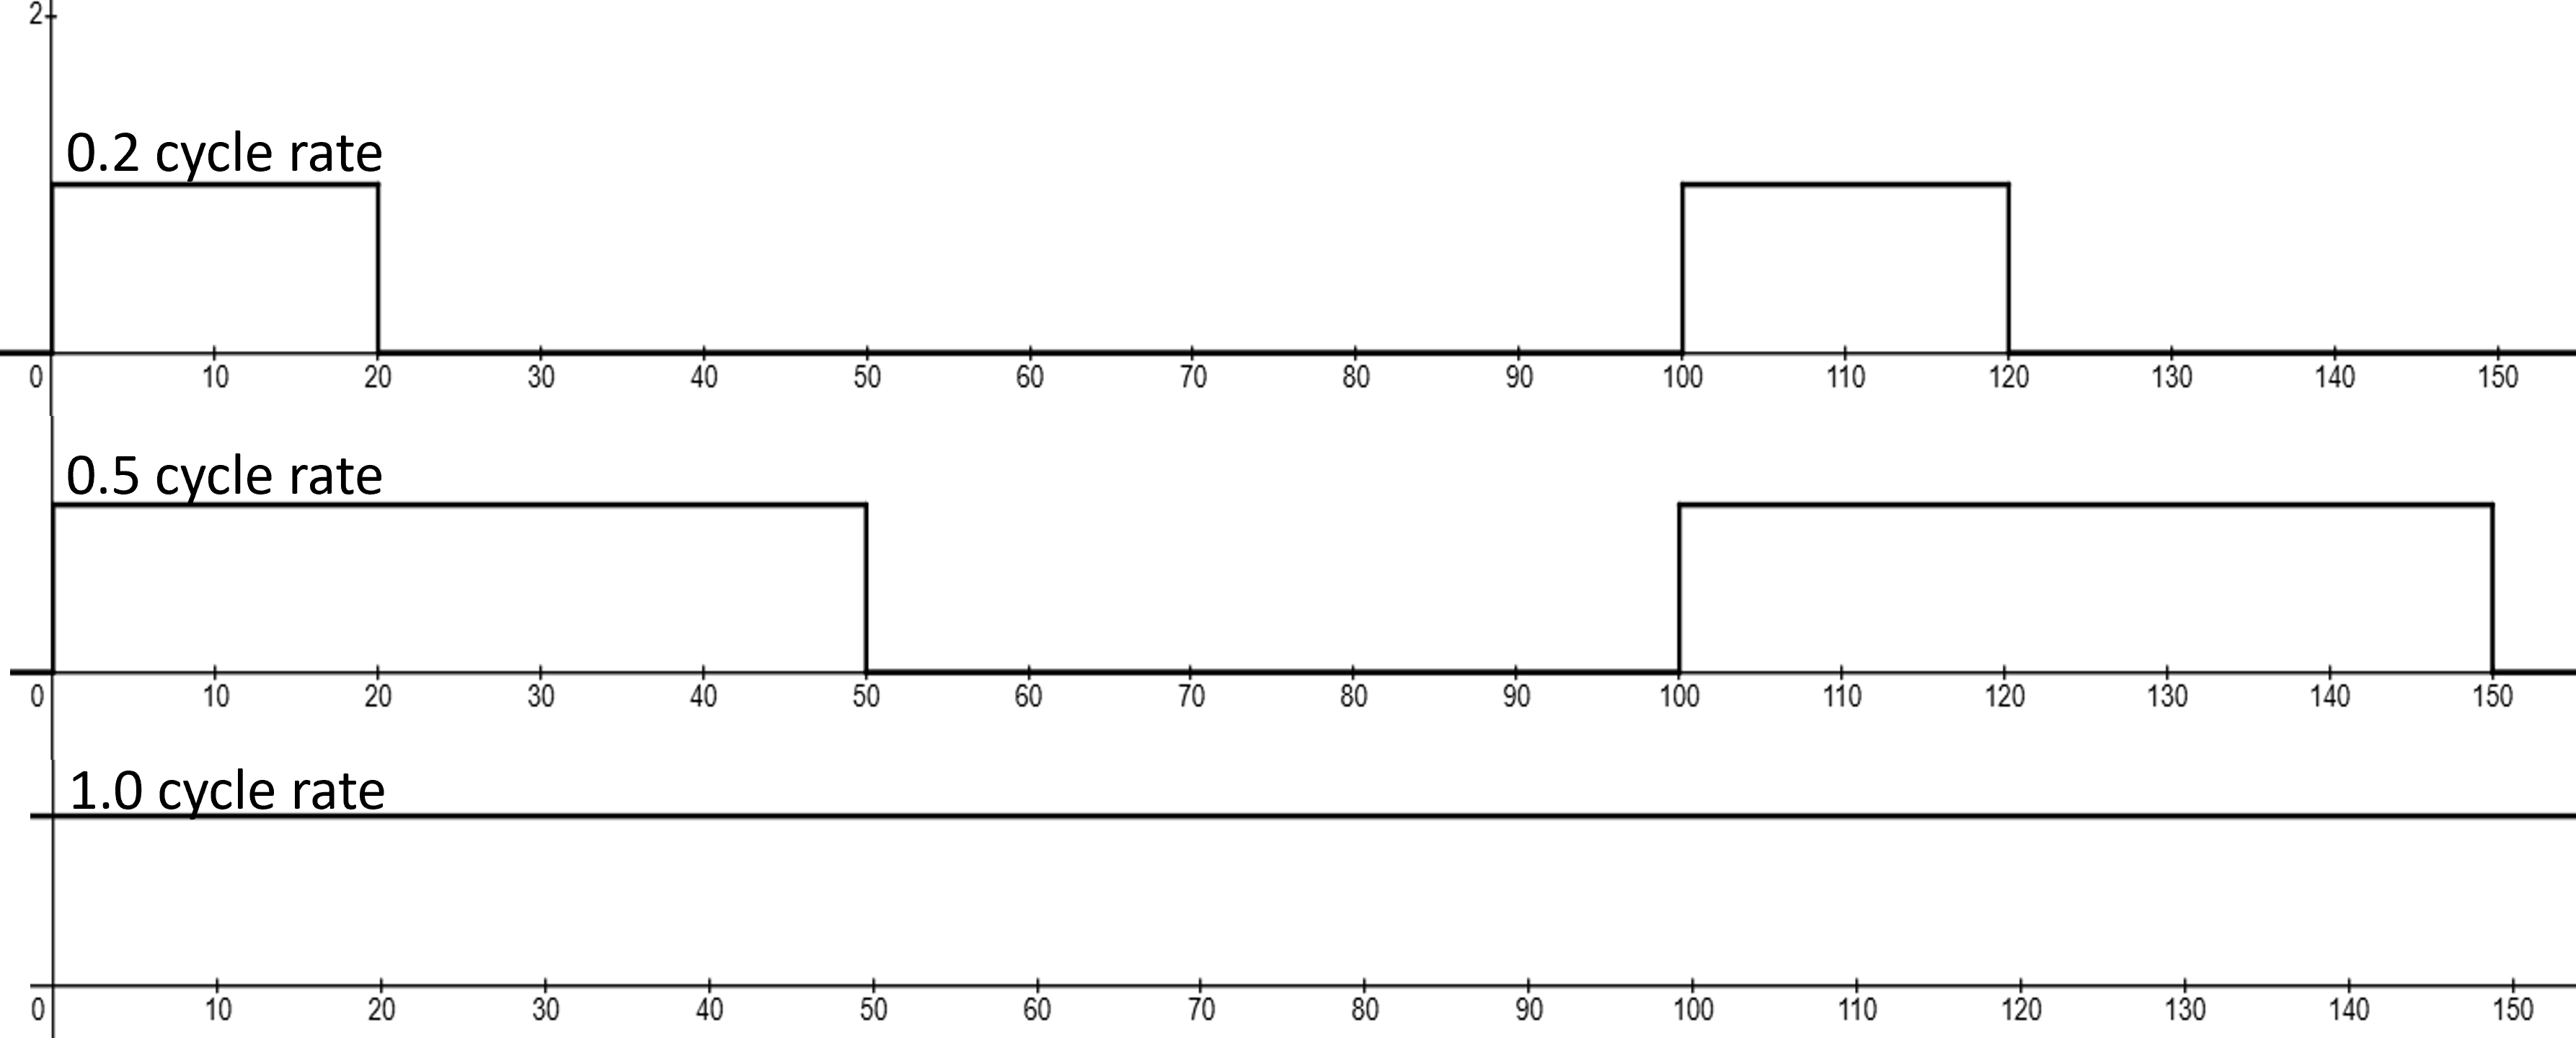
\includegraphics[width=1\textwidth]{Pictures/PWM_3.png}%imagine location
	\caption{PWM with different cycle rates.}\label{fig:pwm_3}%use name for ref.
	
\end{figure}

To simulate differences in texture, the cycle rate—defined as the interval at which the motor alternates between active (vibrating) and inactive (paused) states—was adjusted while maintaining a constant PWM duty cycle. Three distinct cycle rates were designed to represent various virtual textures:

\begin{itemize}
  \item \textbf{Low cycle rate (0.2)}: This is characterized by longer on-off intervals, creating a rough, bumpy tactile sensation.
  \item \textbf{Medium cycle rate (0.5)}: This feature moderates pulse intervals, producing a balanced sensation suitable for medium-textured virtual surfaces.
  \item \textbf{High cycle rate (1.0)}: This involves rapid successive pulses with minimal pauses, resulting in a smooth and continuous tactile impression.
\end{itemize}

This method offers a straightforward yet effective way to represent textural properties by focusing on temporal vibration patterns rather than changing vibration amplitude.
%%%%%%%%

\newpage
\section{Experiment}

\subsection{Experiment 1: Distinguishing Haptic Feedback}
I recruited a total of six participants, all right-handed and aged between 24 and 27 years, for the first experiment. None of the participants had prior experience with the specific haptic device and reported no known sensory or motor impairments. The primary aim of this experiment was to conduct a blind classification test to evaluate their ability to reliably distinguish between three predefined vibration cycle rates: 0.2, 0.5, and 1.0 cycles per second. These cycle rates were chosen to represent three distinct levels of vibration rhythm, intended to simulate variations in virtual surface textures.

Before the formal testing session, all participants went through a familiarization phase where they experienced each of the three cycle rates individually. During this phase, each cycle rate was presented multiple times in a labeled, non-randomized order. This allowed participants to establish a clear tactile reference for the “low,” “medium,” and “high” vibration patterns. Participants were encouraged to ask questions and could repeat the familiarization process as needed to ensure they fully understood each vibration profile before moving on to the blind testing phase. This preparation aimed to minimize learning effects during the main experiment and ensure that the evaluation focused solely on the participants' ability to discriminate tactile sensations.

\textbf{Procedure:} Participants wore and calibrated the glove through repeated hand opening and closing gestures, ensuring accurate hand tracking. Subsequently, participants interacted with a plain white 3D plane in the virtual environment (Figure~\ref{fig:experiment1_setup}), triggering randomly generated vibrations corresponding to one of the three cycle rates. Participants verbally identified the perceived cycle rate after each interaction. Each participant completed 15 randomized trials, assessing their discrimination accuracy.

\begin{figure}[H]\centering
	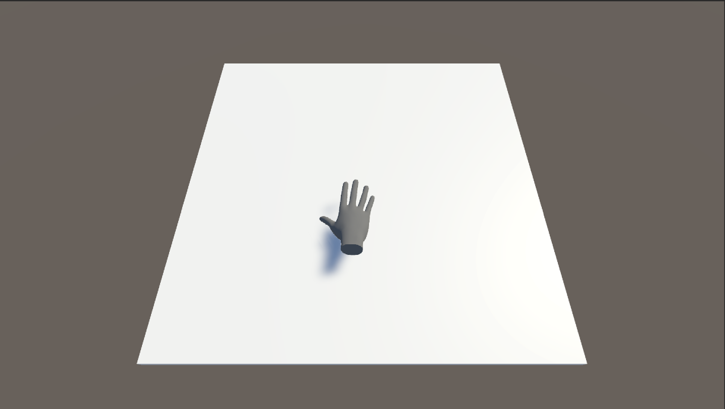
\includegraphics[width=1\textwidth]{Pictures/ex1.png}%imagine location
	\caption{Experimental setup for Experiment~1: participants interacting with a plain white virtual plane to distinguish vibration cycle rates.}\label{fig:experiment1_setup}%use name for ref.
	
\end{figure}

\newpage
\subsection{Experiment 2: Relationship Between Haptic Feedback and Texture Perception}
The participants from Experiment 1 also participated in Experiment 2, ensuring consistency in their experience and enabling a comparative analysis between both experiments. The main objective of this experiment was to investigate the relationship between vibration cycle rates and the perceived realism of textures. It examined how variations in vibrotactile rhythm influenced participants’ subjective interpretations of virtual surface textures. During the experiment, participants interacted with three visually distinct virtual textures—brick, grass, and marble—each carefully selected to represent a range of surface characteristics from rough to smooth.

Each virtual texture was systematically paired with a corresponding vibration cycle rate. The brick texture was linked to the lowest cycle rate (0.2) to represent a coarse, rugged sensation; grass was assigned a medium cycle rate (0.5) to simulate moderate roughness; and marble was paired with the highest cycle rate (1.0) to evoke a smooth and continuous tactile experience. Participants were instructed to touch each virtual texture multiple times using a haptic glove. They were asked to focus on the synchronization between the visual and tactile feedback, noting how accurately the vibration pattern reflected the expected feel of each material.

\textbf{Procedure:} After the first experiment, participants took a 5-minute break before proceeding to the second experiment. In this phase, participants sequentially interacted with each virtual texture (Figure~\ref{fig:experiment2_setup}), experiencing all three vibration cycle rates (0.2, 0.5, and 1.0). After experiencing each set of cycle rates for a given texture, participants selected the cycle rate they felt most accurately matched the visual texture. This procedure was repeated for each texture type for each participant.

\begin{figure}[H]\centering
	\includegraphics[width=1\textwidth]{Pictures/ex2.png}%imagine Avation
	\caption{Experimental setup for Experiment~2: participants interacting with textured virtual planes (brick, grass, marble) to assess vibration realism.}\label{fig:experiment2_setup}
\end{figure}

Collectively, these experiments provided insights into participants' perceptual sensitivity to different vibration cycle rates and evaluated the realism of tactile sensations corresponding to varied virtual textures.

\newpage
\subsection{Post-Experiment Evaluation}
After completing both experiments, participants provided subjective feedback through a questionnaire consisting of 12 statements (Table~\ref{tab:evaluation_questions}). Each statement was rated on a Likert scale from 1 (strongly disagree) to 7 (strongly agree), covering virtual hand embodiment, tactile realism, and immersion. Questions about the sense of virtual hand ownership and control (e.g., Q1, Q3, Q4, Q8) were based on the Virtual Embodiment Questionnaire (VEQ)~\cite{10.1145/3027063.3053272}. Statements assessing how realistic and aligned the tactile sensations felt (Q2, Q6, Q7, Q10) were guided by the Haptic Experience (HX) model~\cite{10.1016/j.ijhcs.2017.04.004}. Additionally, overall immersion (Q12) was evaluated according to concepts from the Presence Questionnaire (PQ)~\cite{10.1162/105474698565686}.

\begin{table}[htbp]
    \centering
    \caption{Post-experiment evaluation questionnaire.}
    \label{tab:evaluation_questions}
    \resizebox{\textwidth}{!}{
    \begin{tabular}{c | c}
        \hline
        \textbf{Question} & \textbf{Statement}\\
        \hline
        Q1 & I felt as if the virtual hands were my own.\\\hline
        Q2 & I felt that the tactile sensations were caused by the virtual hand.\\\hline
        Q3 & I felt as if my hand were the virtual hand.\\\hline
        Q4 & I felt like I was controlling the movement of the virtual hand.\\\hline
        Q5 & I felt as if the virtual hand was naturally connected to my body.\\\hline
        Q6 & The tactile sensations I perceived felt naturally aligned with the virtual hand.\\\hline
        Q7 & When I touched the virtual plane, I felt as if my real hand was also being touched.\\\hline
        Q8 & The movements of the virtual hand felt natural to me.\\\hline
        Q9 & I felt that the virtual hand responded as expected to my movements.\\\hline
        Q10 & I had the sensation that I could feel the texture of objects through the virtual hand.\\\hline
        Q11 & I felt a mismatch between my real hand and the virtual hand.\\\hline
        Q12 & The overall experience made me feel immersed in the virtual environment.\\
        \hline
    \end{tabular}}
\end{table}

Participant responses provided qualitative insights into embodiment, tactile realism, and immersion, complementing the quantitative outcomes from Experiments~1 and 2.



% The results of two preceding experiments are applied to design a simulation. The time-dependent synced-rotational gain of 1.6 degrees per second and the curvature distance of 23cm at the distance of 4m (walking speed 0.5m/s x walking duration 8s) are employed to simulate the walking path of an agent. An agent walks at the speed of 0.5m/s and changes the direction where he/she walks for a randomly selected direction between 0 to 360 degrees every 4 seconds. The shoulder with of the agent is 46cm.



% As for the physical area where agents walk, three patterns of Large, Medium, and Small are taken into consideration by referring to~\cite{PMID:18183898}. Large is an area of 21.375 x 15.075m, Medium is 28.5 x 20.1m and Small is 35.625 x 25.125m. An agent collides with a surrounding wall when the distance between the wall and the center of the agent is less than 23cm. The agent also collides with other agents when their center-to-center distance less than 46cm. When agents collide with others, the 2:1 turn~\cite{8798319} strategy is performed to resolve starvation. As for collision avoidance, the likelihood of colliding between agents is obtained by a collision prediction bar. A collision prediction bar is 4m long and its origin is placed at the center of each agent. Its direction comes from a linear regression line which is obtained from the path he/she walked past 8 seconds. A collision is predicted if two collision prediction bars overlap, and the given collision avoidance of the Holm's method and the proposed one is performed. The time-dependent rotational gain for the Holm's method and the time-dependent synced-rotational gain for the proposed method are set the same with 1.6deg/s and the duration is 8 seconds.

% \newpage

% Fig.~\ref{fig:Simulation_2} to Fig.~\ref{fig:Simulation_15} show some screenshots of the simulation. The colored dots indicate agents. The outer circle of the dot indicates their shoulder width of 46cm. The triangle on the dot indicates their facing direction.

% \begin{figure}[H]\centering
% 	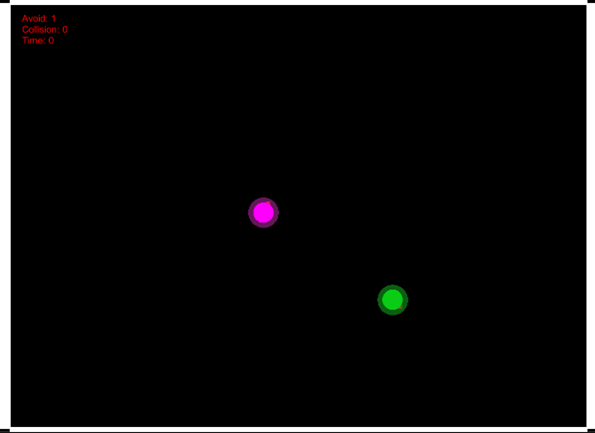
\includegraphics[width=0.9\textwidth]{Pictures/two users share real space.png}%imagine location
% 	\caption{Simulation for two users.}\label{fig:Simulation_2}%use name for ref.
	
% \end{figure}


% \begin{figure}[H]\centering
% 	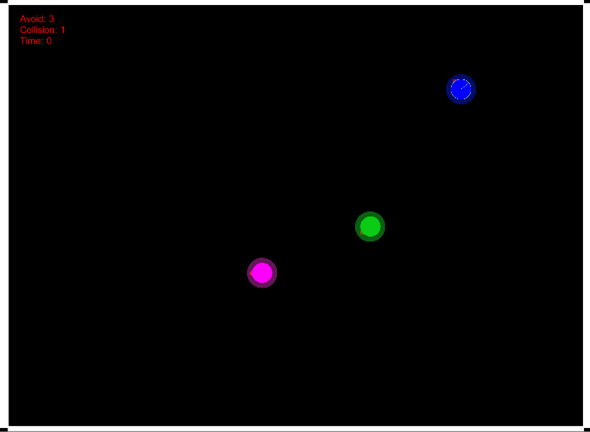
\includegraphics[width=0.9\textwidth]{Pictures/three users share real space.png}%imagine location
% 	\caption{Simulation for three users.}\label{fig:Simulation_3}%use name for ref.
	
% \end{figure}


% \begin{figure}[H]\centering
% 	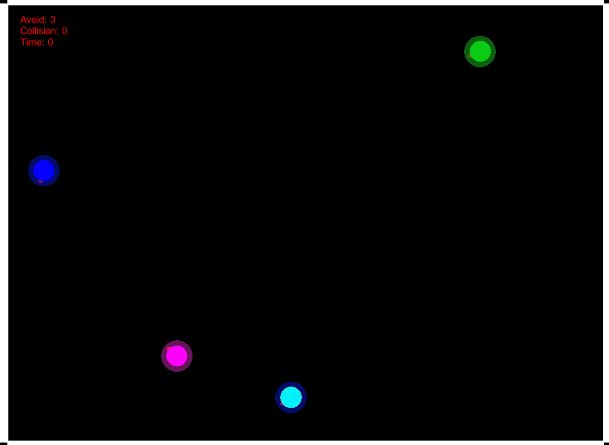
\includegraphics[width=0.9\textwidth]{Pictures/four users share real space.png}%imagine location
% 	\caption{Simulation for four users.}\label{fig:Simulation_4}%use name for ref.
	
% \end{figure}


% \begin{figure}[H]\centering
% 	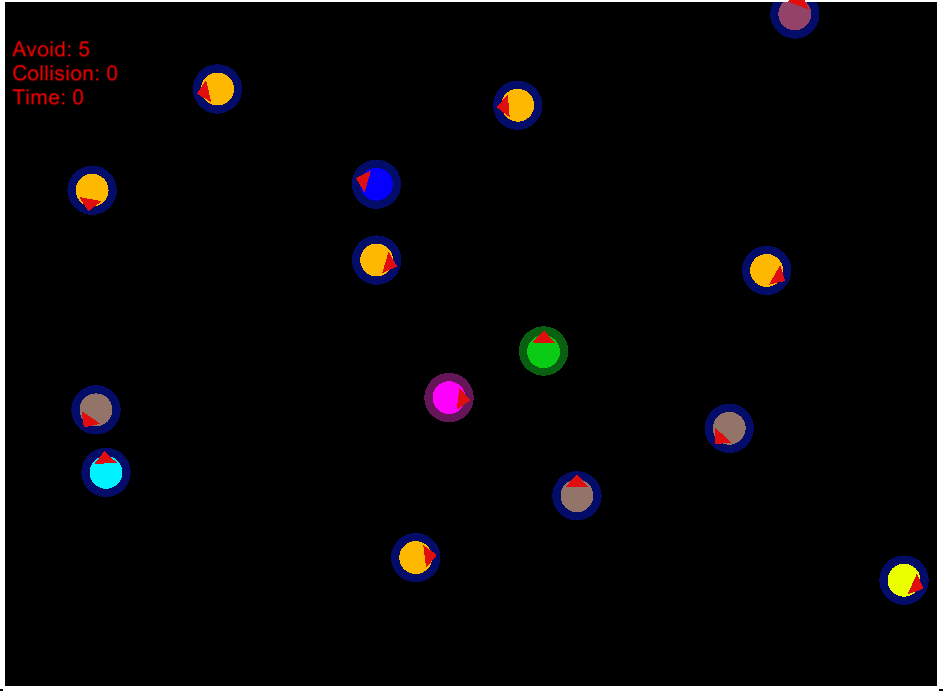
\includegraphics[width=0.9\textwidth]{Pictures/fifteen users share real space.png}%imagine location
% 	\caption{Simulation for fifteen users.}\label{fig:Simulation_15}%use name for ref.
	
% \end{figure}

% \newpage

% \begin{table}[h!]\centering
% 	\caption{Data Collection.}
% 	\label{tab:Data CollectionEx3}%\scriptsize
% 		\scalebox{1.0}{
% 	\begin{tabular}{ |p{4cm}|p{3cm}|p{6cm}|}
% 	\hline
% 		Variable & Unit & Description \\\hline
% 		Count of avoidance & count &Number of occasions that a collision with other agents are successfully avoided.\\\hline
% 		Count of collision & count & Number of collisions with other agents that occur during the trial.\\\hline
		
		
% 	\end{tabular}
% 	}
% \end{table} 

%  A series of simulation is conducted under the following conditions. 14 patterns of agents (2$\sim$15) x 3 physical areas (Large, Medium and Small) x 10 trials x 2 methods = 840 trials in all. The data to be collected during each trial is summarised in Table.~\ref{tab:Data CollectionEx3}.

% \newpage

% \section{Results}
% Fig.~\ref{fig:Area of 75 Percent} to Fig.~\ref{fig:Area of 125 Percent} show both the count of collisions and count of avoidance. The horizontal axis is the number of agents and the vertical one is the number of counts. The red line shows data from the Holm's method and the blue line shows data from the proposed method. The dash line is the count of collisions and the solid line is the count of avoidance. The three figures draw those lines at each different size of physical areas: Small, Medium and Large. From the results, it seems that as the area is larger, the counts of collisions and avoidance are reduced. Additionally, across all the number of agents for all the size of physical areas, the count of collisions for the proposed method is lower than the Holm's one.


% Fig.~\ref{fig:Performance of the number of collisions} and Fig.~\ref{fig:Performance Averages} show a comparative improvement of the proposed method to the Holm's method. The horizontal axis is the number of agents and the vertical one is the percentage of the count of collisions from the proposed method for the one from the Holm's method at each different size of area (if the percentage is 100 percent, it means no improvement.) At Large area, an average of ratio is 80.22 percent. Fig.~\ref{fig:Performance Averages} shows the average and its standard deviation across all the number of agents at each different size of area.

% Fig.~\ref{fig:Average of count of collisions} shows the average of counts of collisions at each different size of area for each method across all the number of agents. From the graph, there is a significant difference in the count of collisions between the Holm's method and proposed one for Medium and Large areas.  Fig.~\ref{fig:Average of count of collisions avoidance} shows the average of counts of avoidance at each different size of area for each method across all the number of agents. From the graph,  there is a significant difference in the count of  avoidance between the two methods for all the sizes of areas. The details of statistical evaluation are found in Appendix \ref{appendix:d} and Appendix \ref{appendix:e}.

% Fig.~\ref{fig:Collision times average in all areas of our method} shows the average of counts of collisions at each the number of agents for each method across different sizes of areas. The count of collisions decreases after applying the proposed method over all the number of agents.  Fig.~\ref{fig:Avoidance times average in all areas of our method} indicates the average of counts of avoidance at each the number of agents for each method, the agents can avoid collisions better by 44.37\% in comparison with the Holm's method.

% \newpage

% \begin{figure}[H]\centering
% 	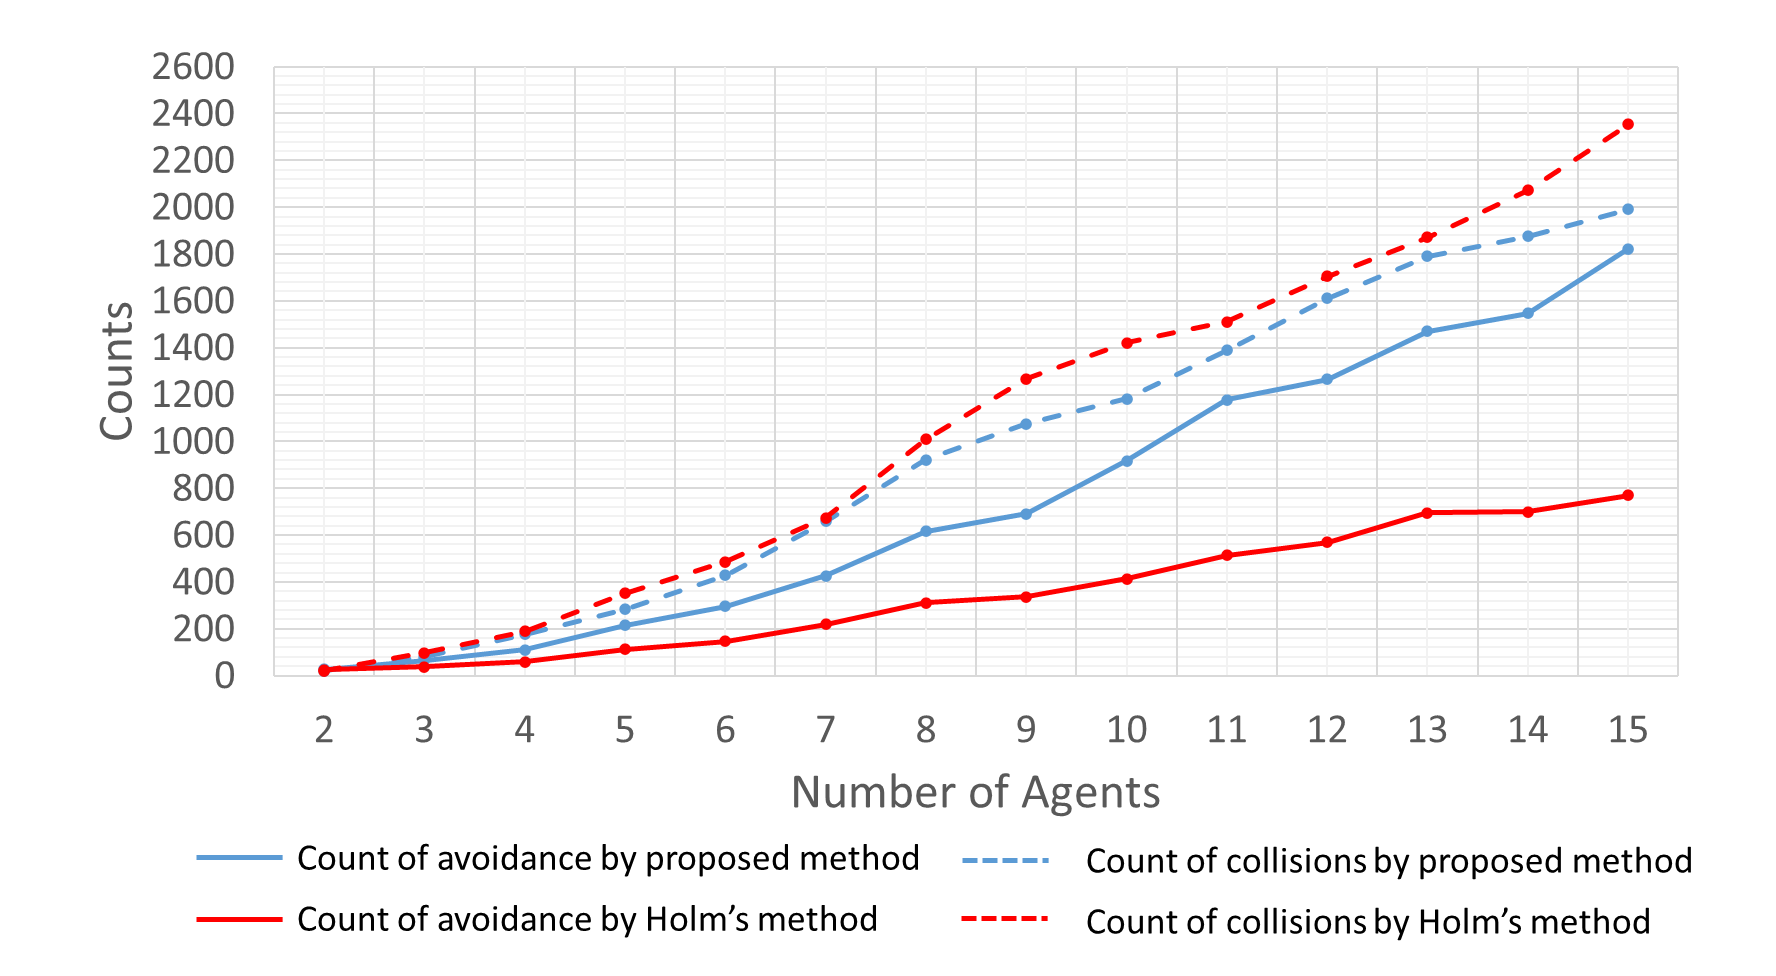
\includegraphics[width=1.0\textwidth]{Pictures/Area of 75 Percent.png}%imagine location
% 	\caption{Performance of collision avoidance for Small area.}\label{fig:Area of 75 Percent}%use name for ref.
	
% \end{figure}

% \begin{figure}[H]\centering
% 	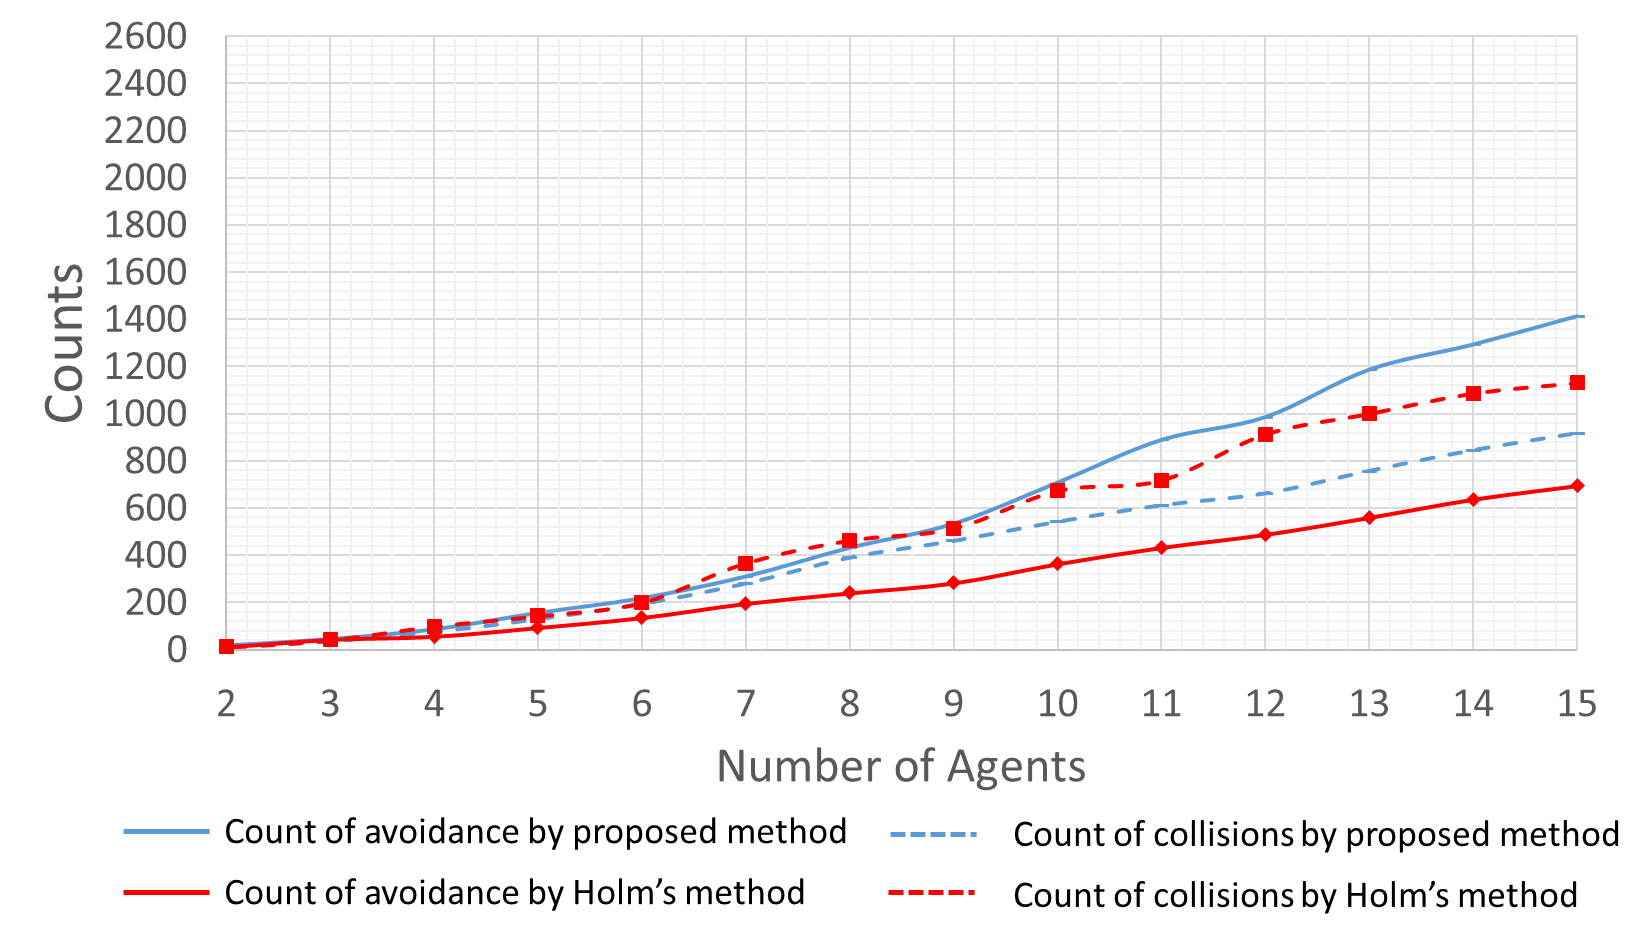
\includegraphics[width=1.0\textwidth]{Pictures/Area of 100 Percent.png}%imagine location
% 	\caption{Performance of collision avoidance for Medium area.}\label{fig:Area of 100 Percent}%use name for ref.
	
% \end{figure}

% \begin{figure}[H]\centering
% 	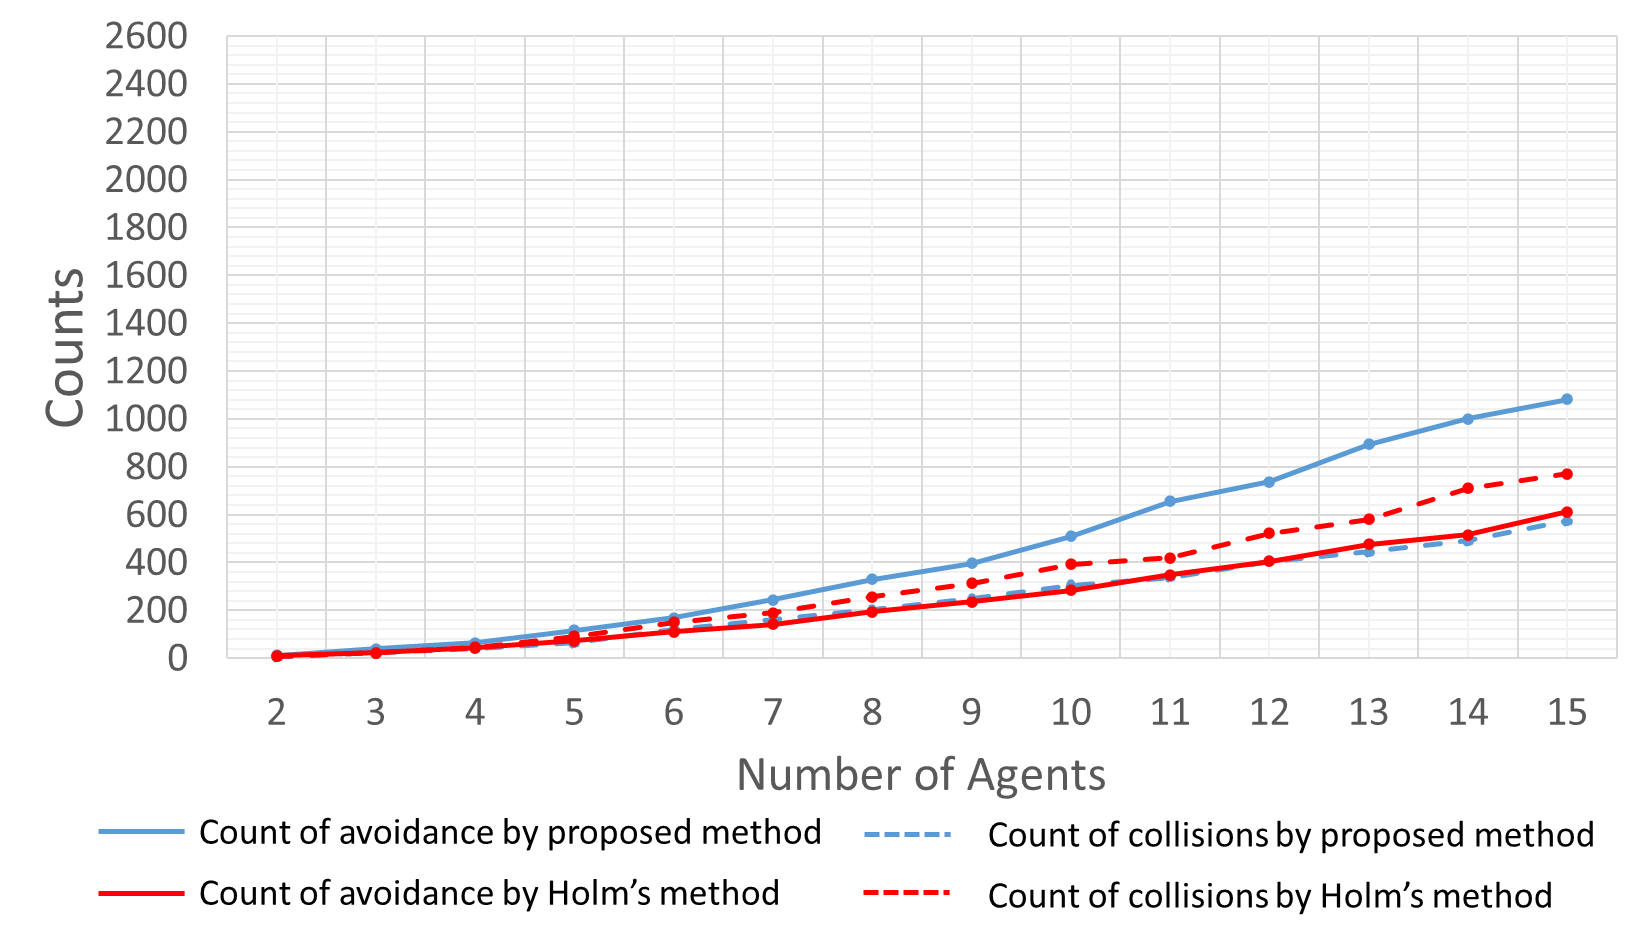
\includegraphics[width=1.0\textwidth]{Pictures/Area of 125 Percent.png}%imagine location
% 	\caption{Performance of collision avoidance for Large area.}\label{fig:Area of 125 Percent}%use name for ref.
	
% \end{figure}
% \newpage
% \begin{figure}[H]\centering
% 	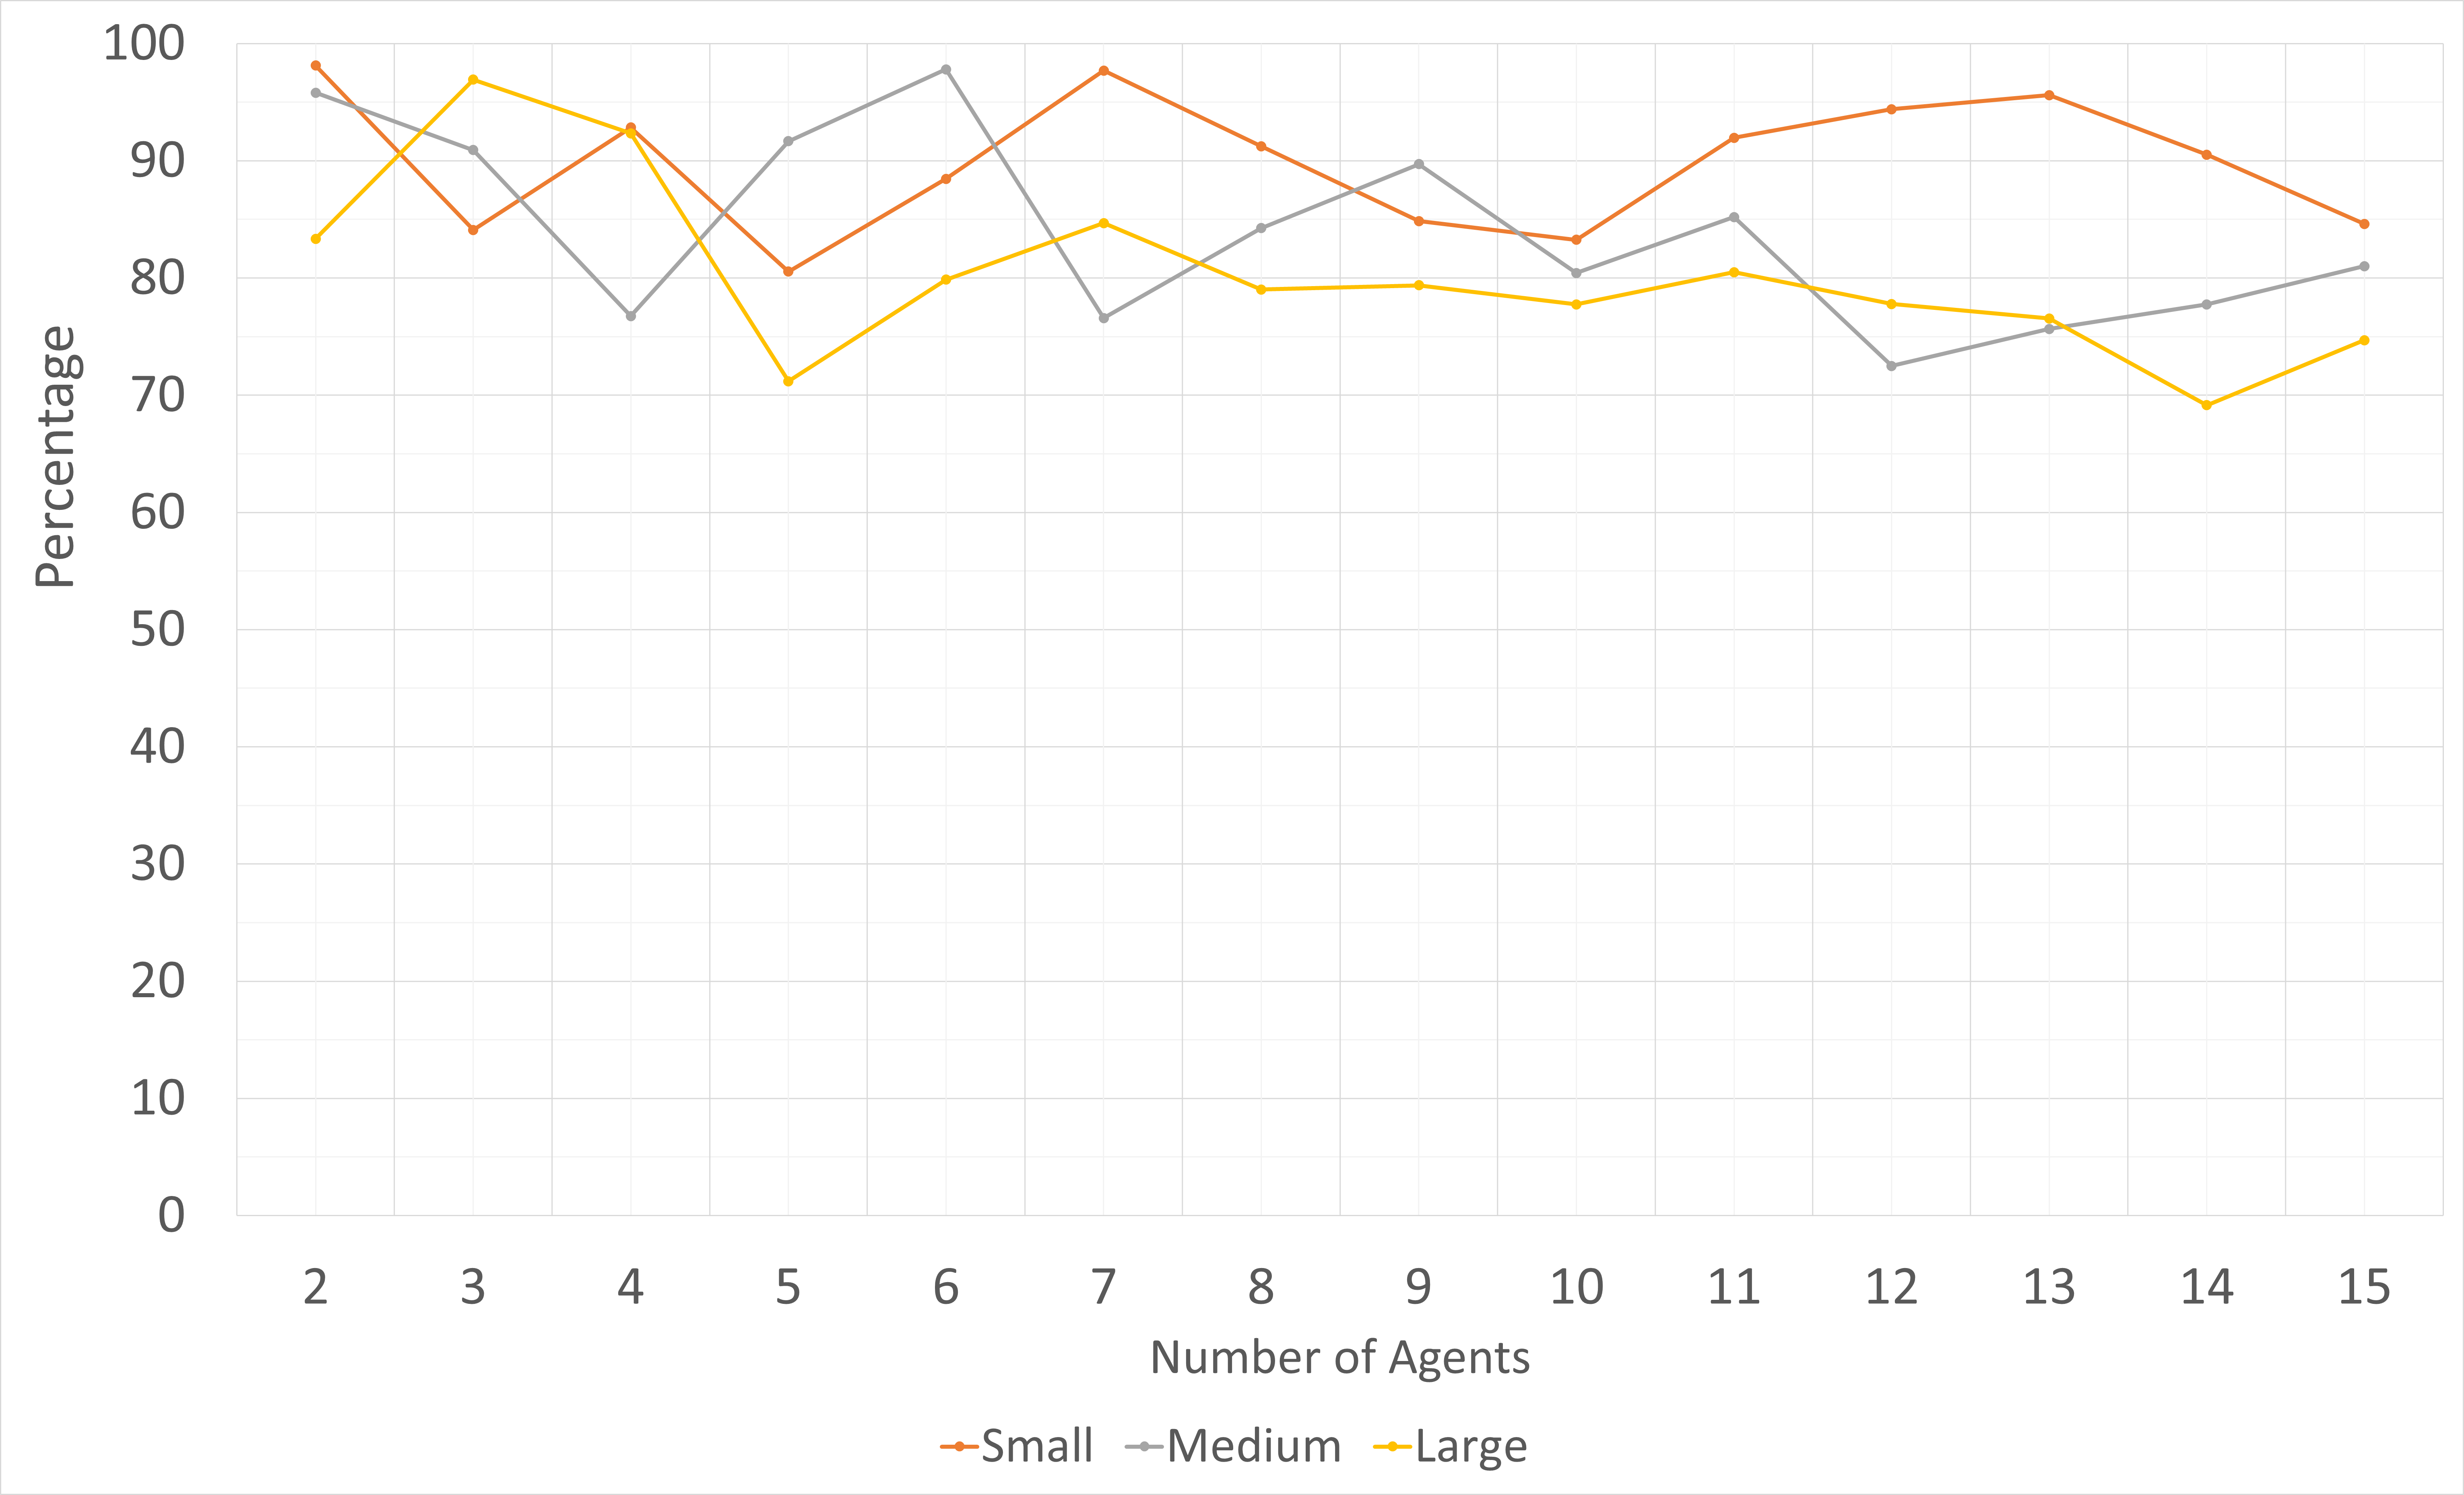
\includegraphics[width=1.0\textwidth]{Pictures/Performance of the number of collisions.png}%imagine location
% 	\caption{Improvement of the proposed method for the Holm's method in terms of the count of collisions.}\label{fig:Performance of the number of collisions}%use name for ref.
	
% \end{figure}
% \begin{figure}[H]\centering
% 	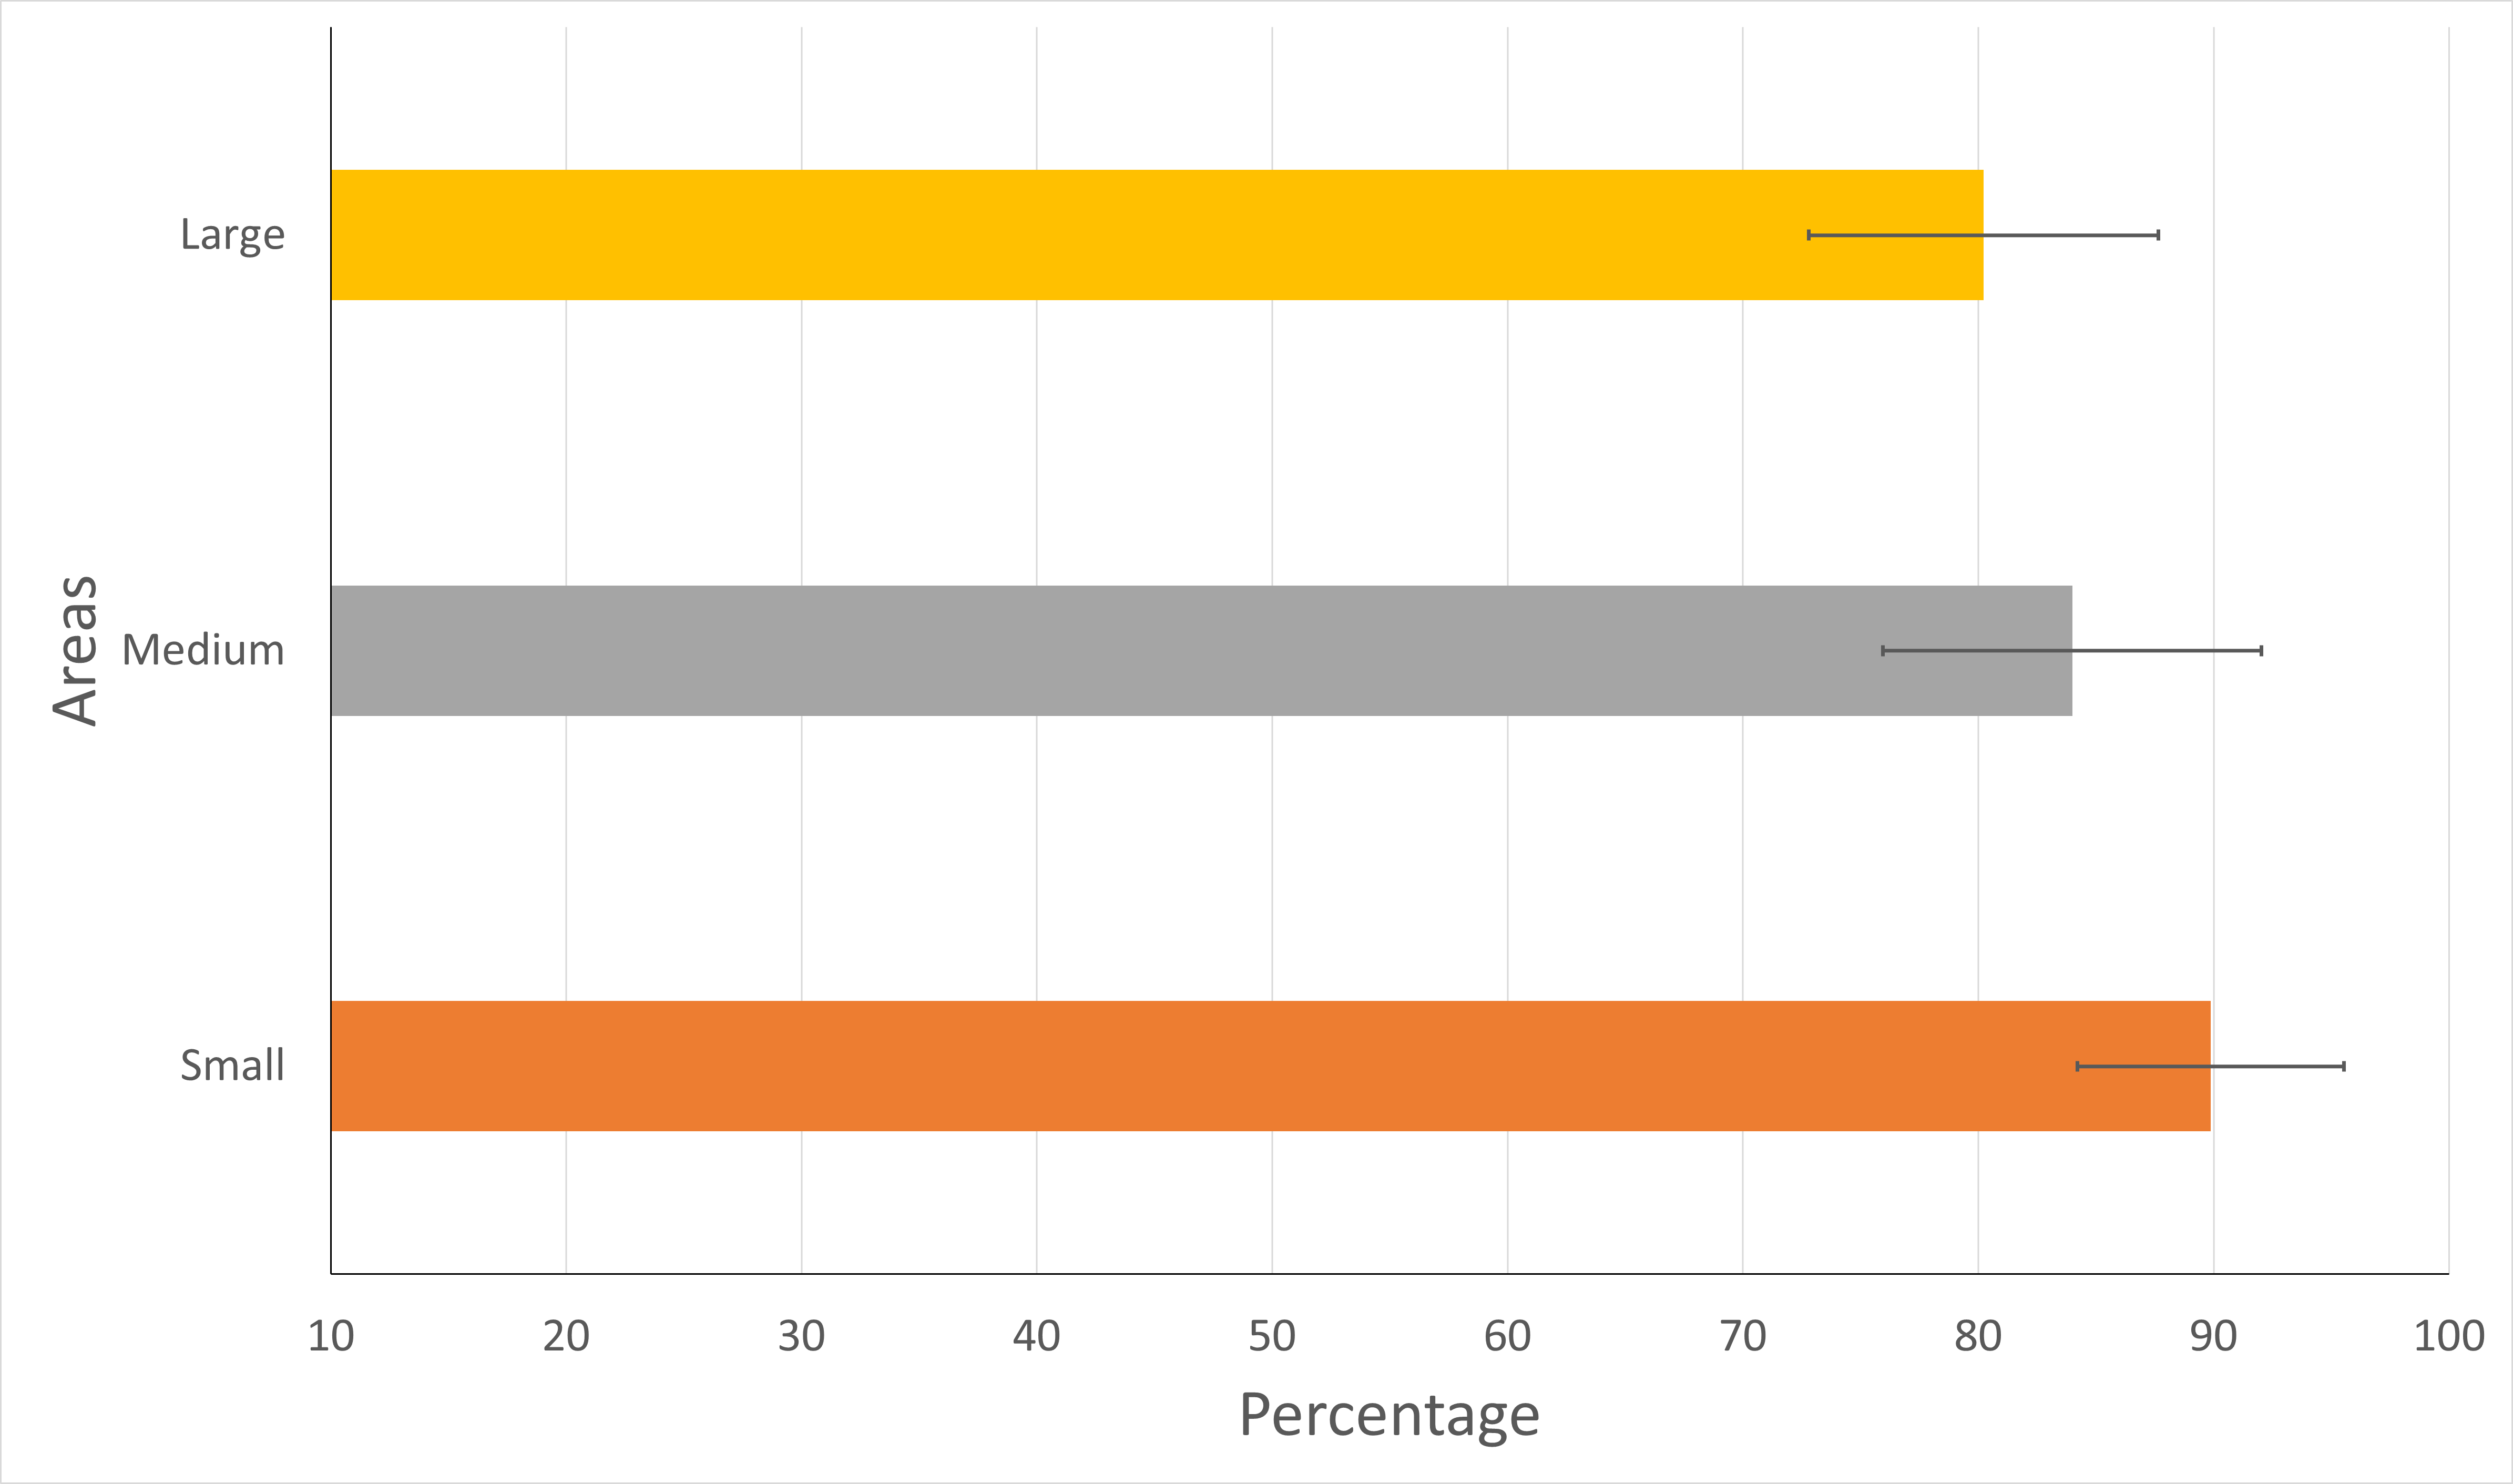
\includegraphics[width=1.0\textwidth]{Pictures/Performance Averages.png}%imagine location
% 	\caption{Average of the improvement.}\label{fig:Performance Averages}%use name for ref.
	
% \end{figure}


% \begin{figure}[H]\centering
% 	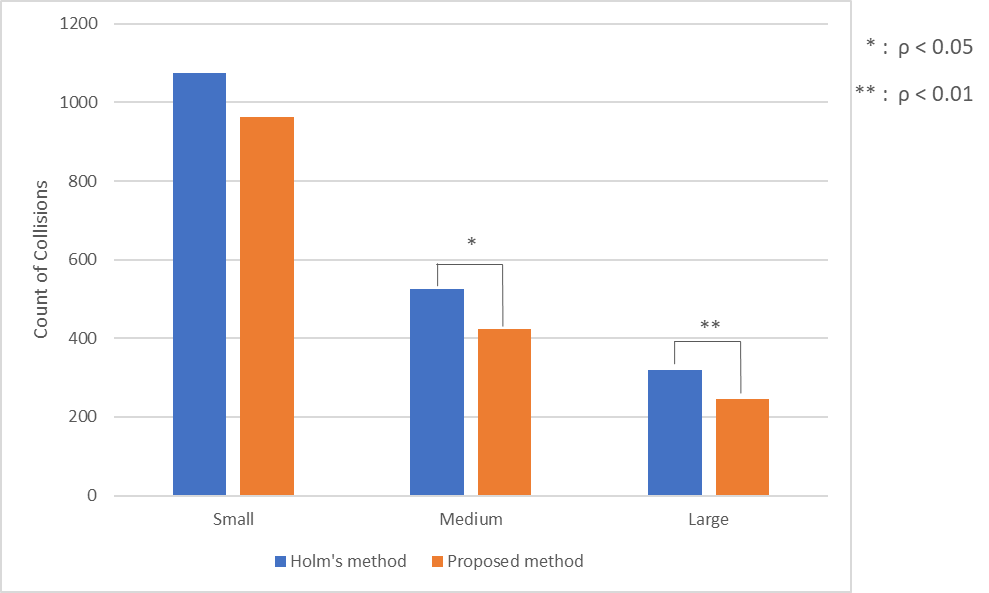
\includegraphics[width=1.0\textwidth]{Pictures/Average of count of collisions of each different of area.png}%imagine location
% 	\caption{Average of counts of collisions at each different size of area.}\label{fig:Average of count of collisions}%use name for ref.
	
% \end{figure}
% \begin{figure}[H]\centering
% 	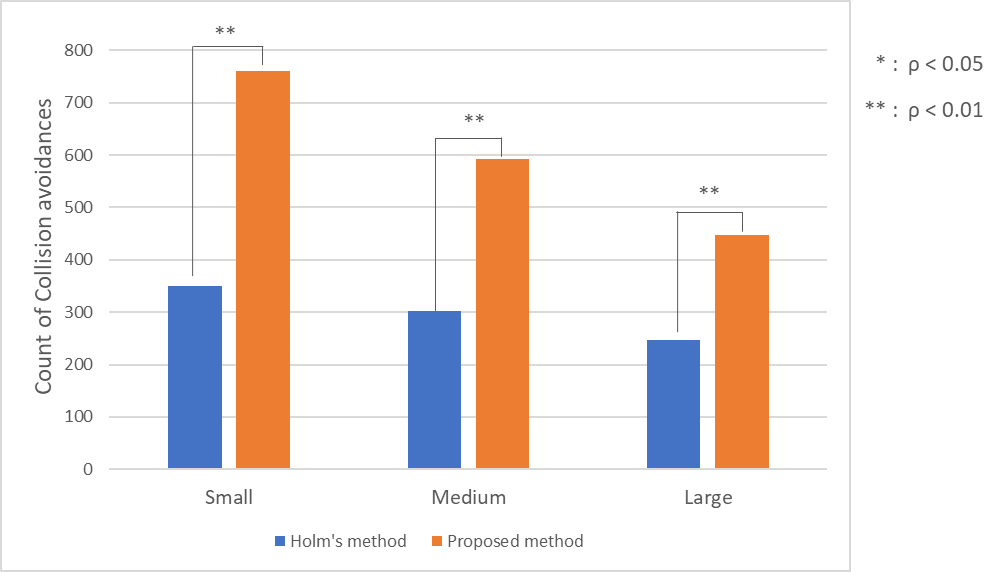
\includegraphics[width=1.0\textwidth]{Pictures/Average of count of avoidance of each different of area.png}%imagine location
% 	\caption{Average of counts of avoidance at each different size of area.}\label{fig:Average of count of collisions avoidance}%use name for ref.
	
% \end{figure}
% %\newpage




% \begin{figure}[H]\centering
% 	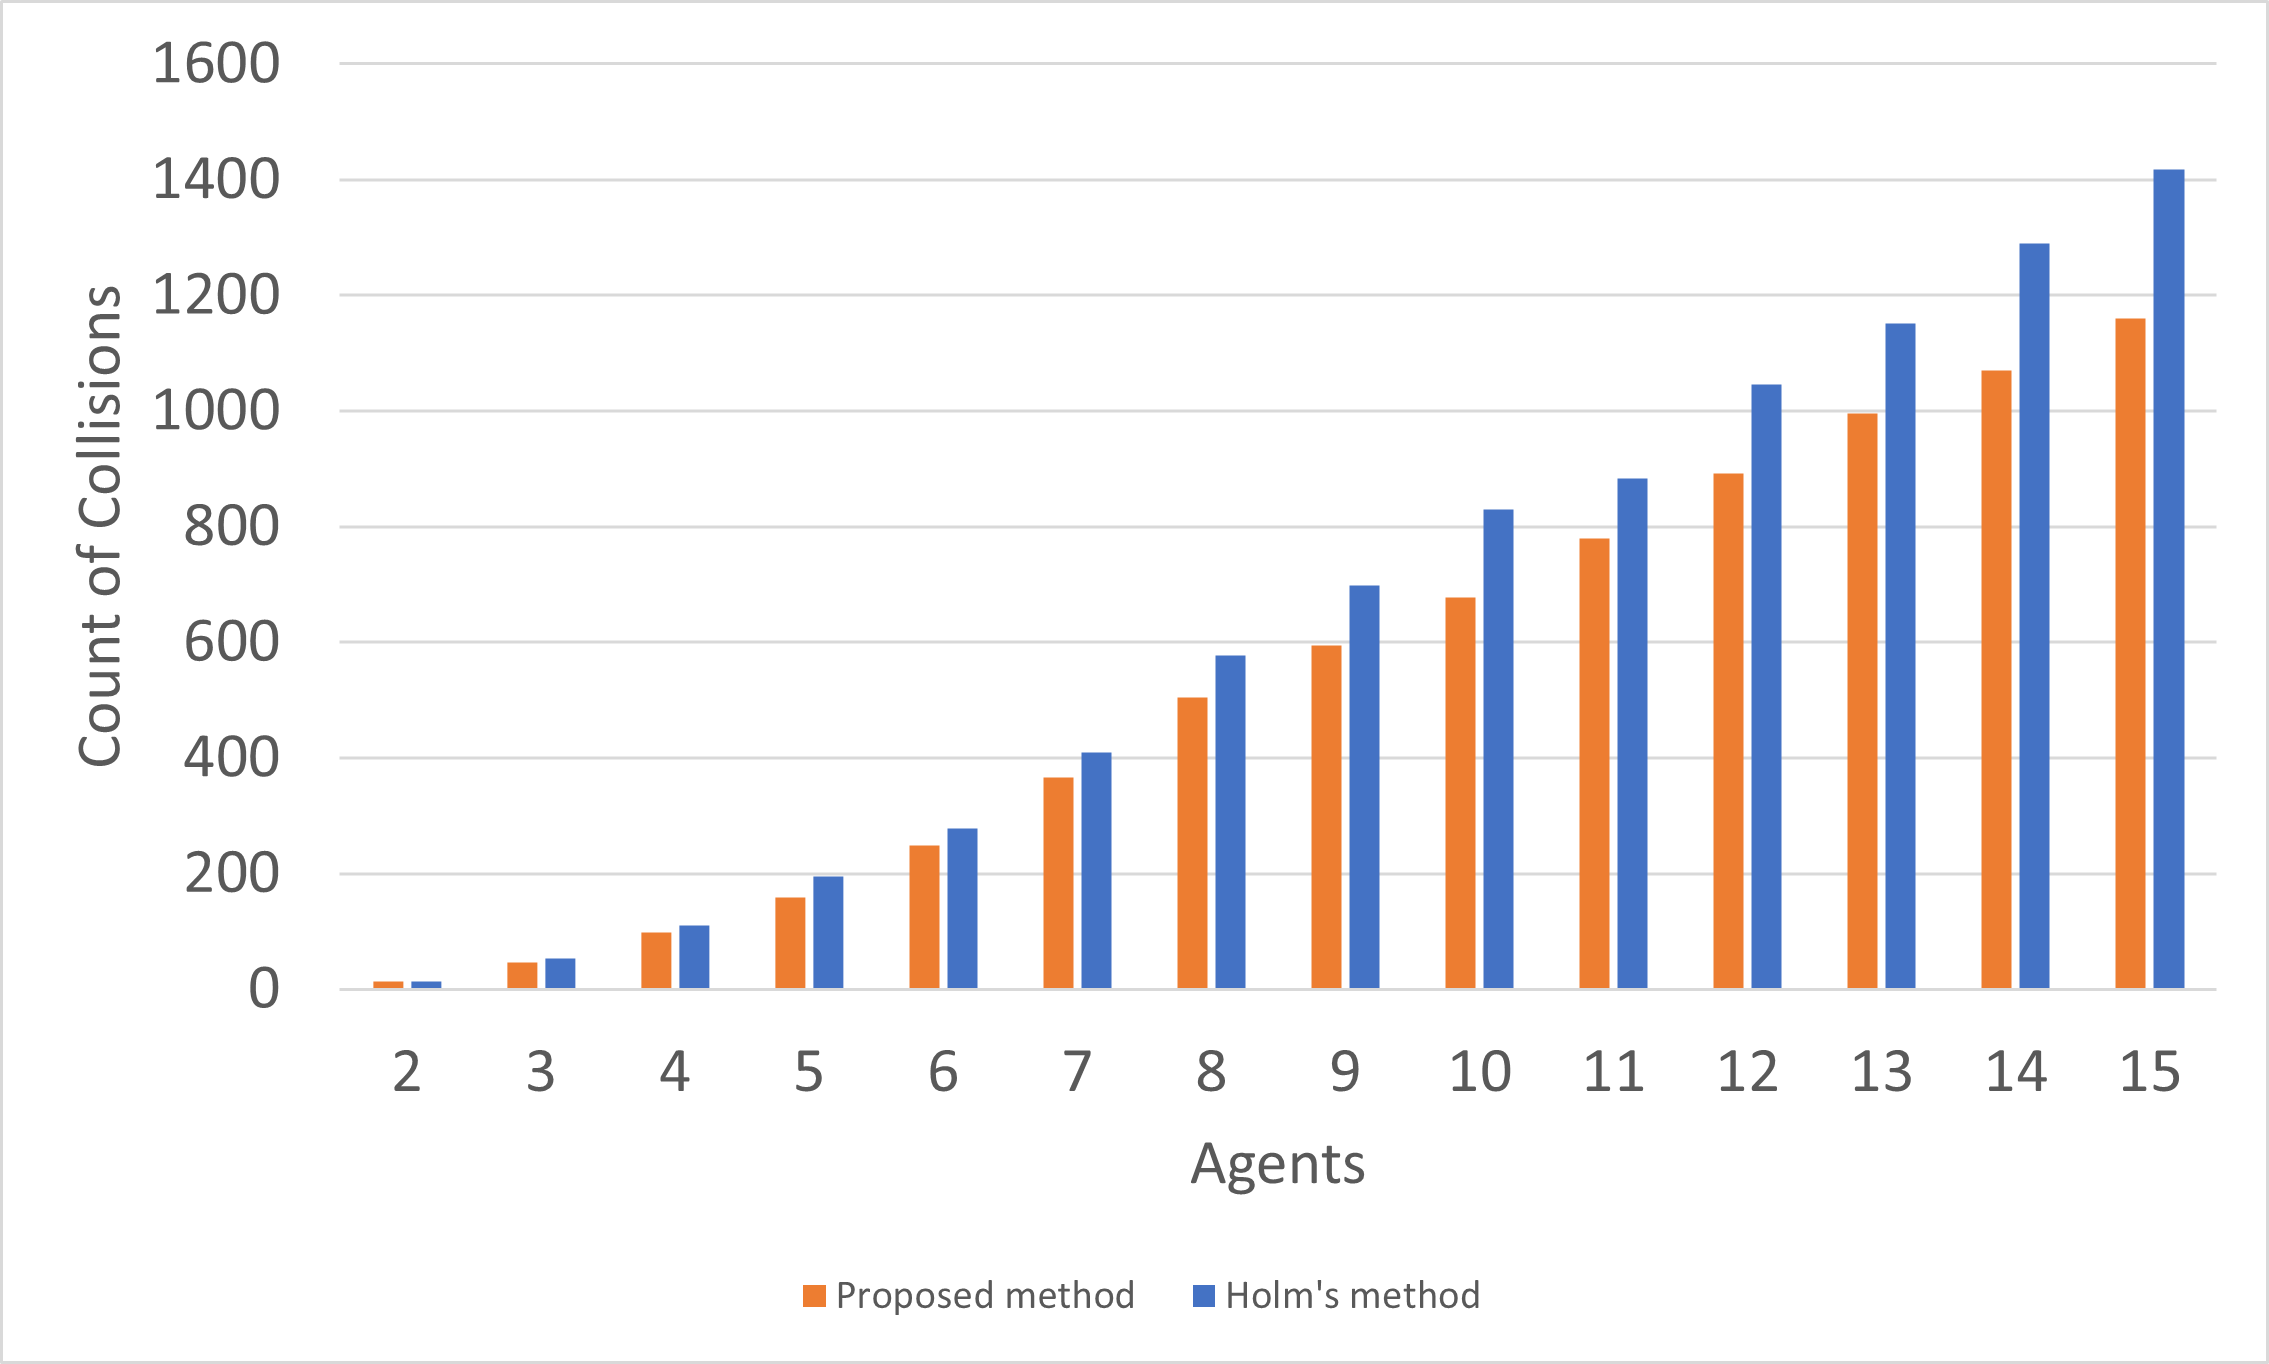
\includegraphics[width=1.0\textwidth]{Pictures/Average of count of collision of across all the number of user.png}%imagine location
% 	\caption{Average of counts of collisions at each the number of agents for each method.}\label{fig:Collision times average in all areas of our method}%use name for ref.
	
% \end{figure}
% \begin{figure}[H]\centering
% 	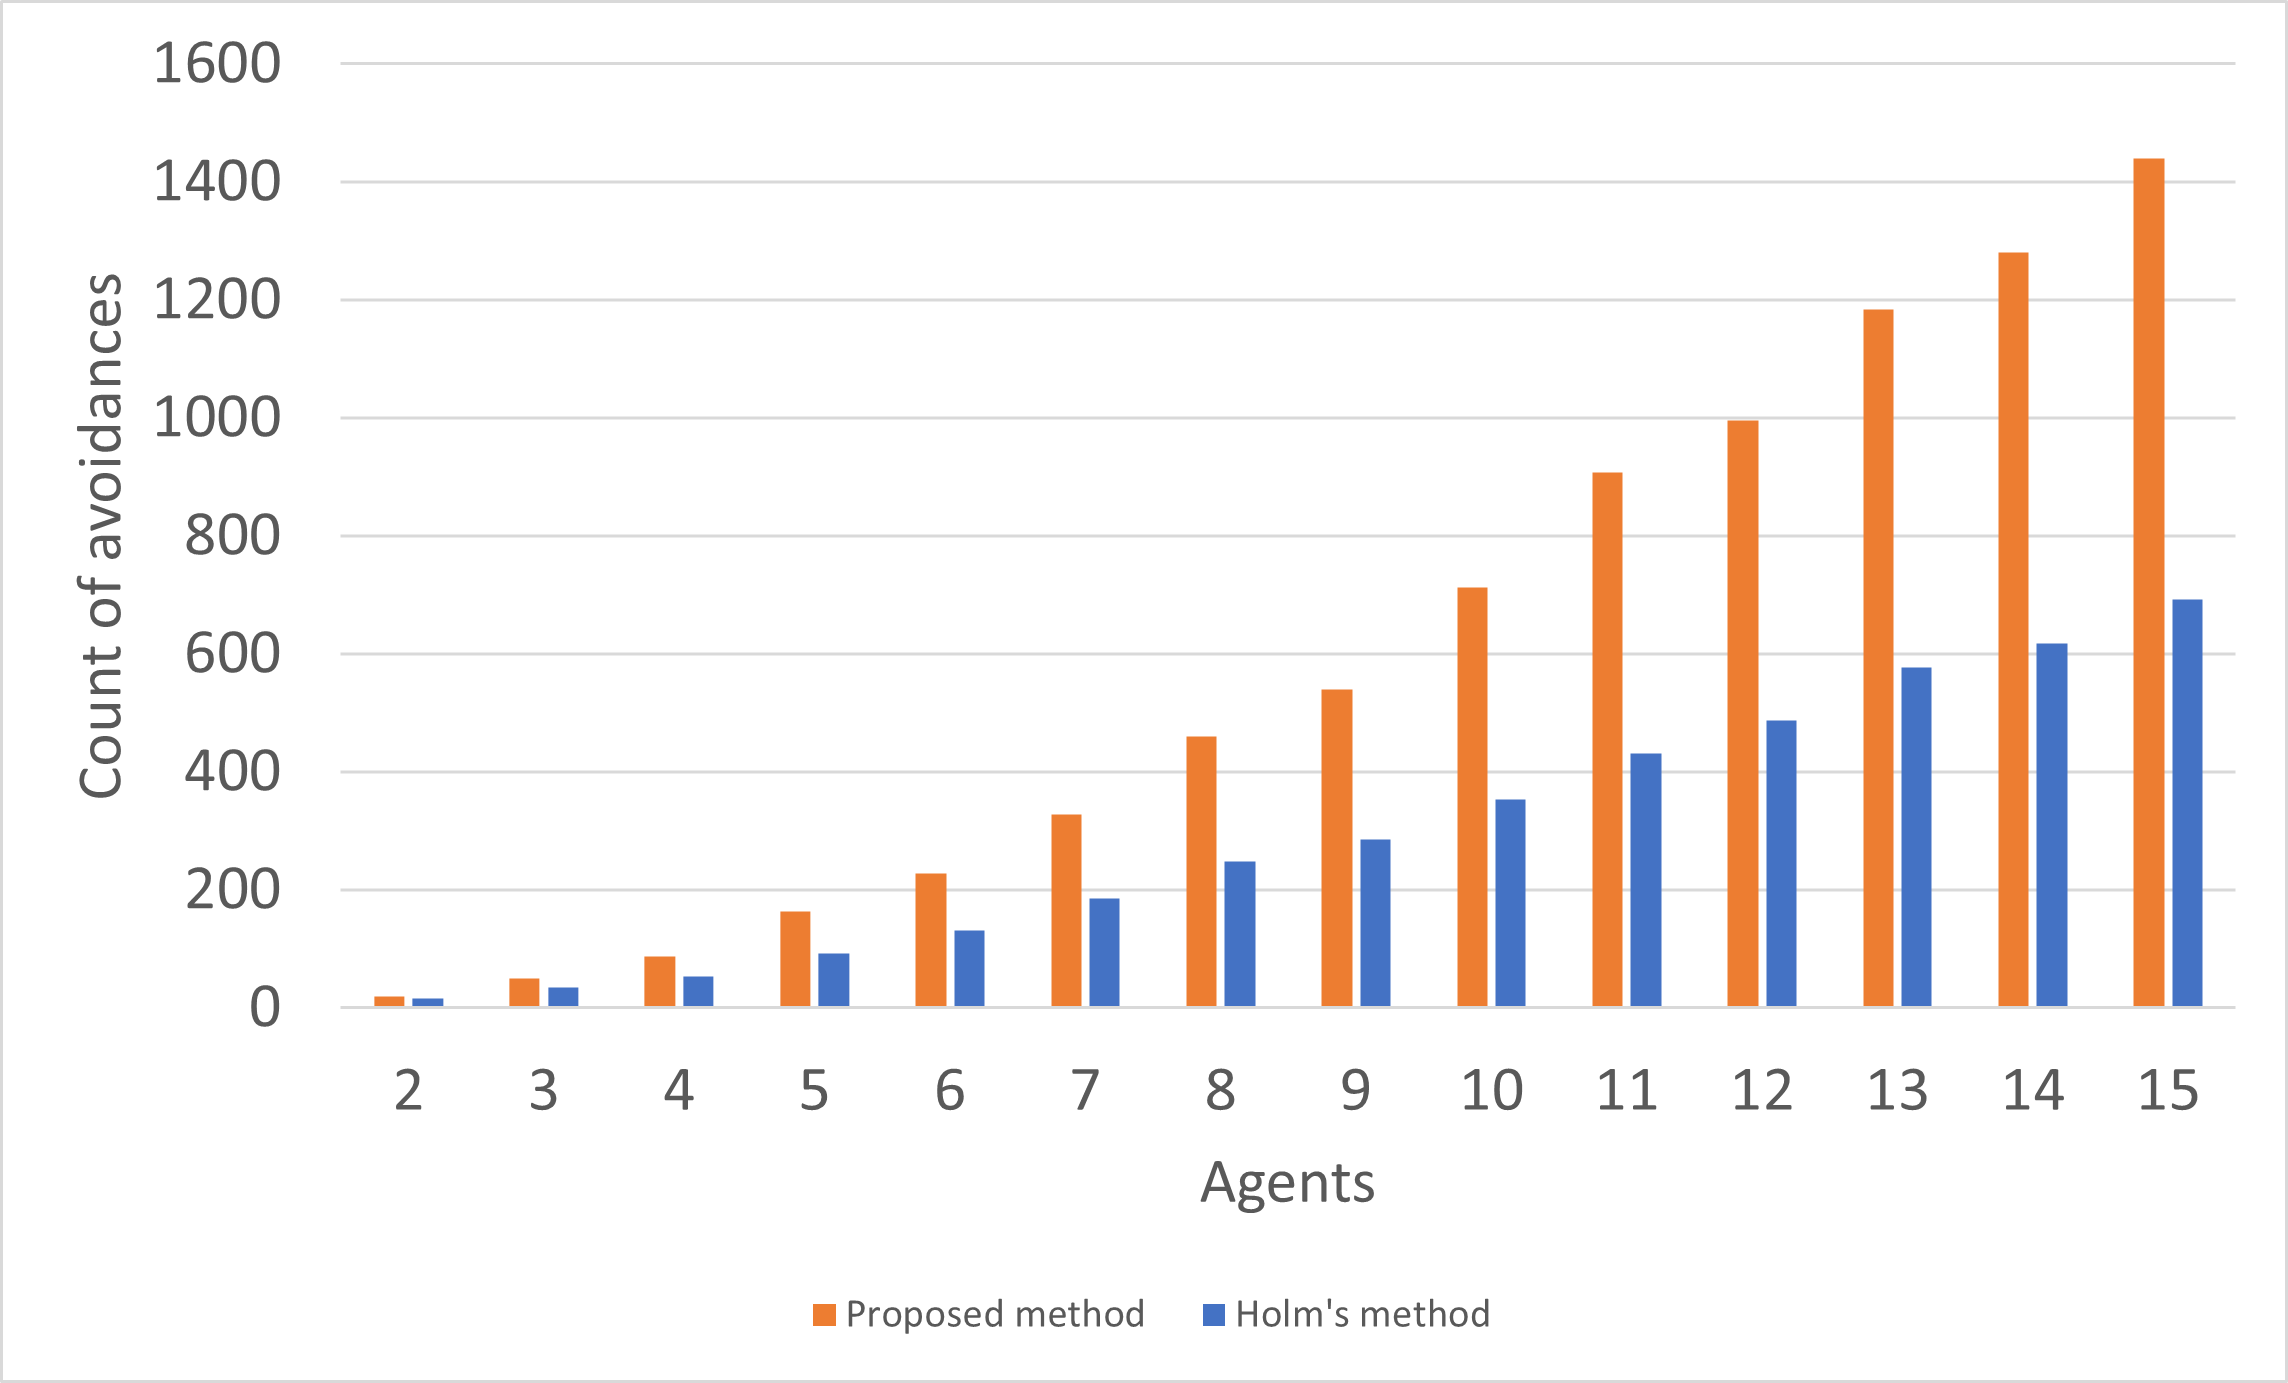
\includegraphics[width=1.0\textwidth]{Pictures/Average of count of collision avoidance of across all the number of user.png}%imagine location
% 	\caption{Average of counts of avoidance at each the number of agents for each method.}\label{fig:Avoidance times average in all areas of our method}%use name for ref.
	
% \end{figure}




